\chapter{Implementazione}

L'implementazione deve rappresentare una simulazione deterministica. Per questo motivo non sono stati usati tread (oggetti Java \texttt{Thread}), la gestione del tempo avviene in modo discreto.

%%%%%%%%%%%%%%%%%%%%%%%%%%%%%%%%%%%%%%%%%%%%%%%%%%%%%%%%%%%%
\section{Scheduler}
Ogni possibile implementazione di un algoritmo di scheduling è un'estensione della classe \texttt{Scheduler}. Questo permette di definire i comportamenti comuni a tutti gli scheduler e di astrarre future implementazioni.

Per l'implementazione, oltre a ciò che definisce uno scheduler (i.e., taskSet e l'eventuale protocollo di accesso alle risorse), è stato necessario mantenere una lista di task pronti \texttt{readyTaskse} una di task bloccati \texttt{blockedTask}. Inoltre è necessario mantenere un riferimento all'ultimo task che è andato in esecuzione.

\myskip

L'implementazione della logica di scheduling è la stessa sia per RM che per EDF: il metodo \texttt{schedule} con i metodi healper necessari sono stati, per questo motivo, inseriti all'interno della classe base. Ogni implementazione concreta deve sono definire alcuni aspetti usati poi nella logica. Per modellare questo principio è stato usato il Template Mehod pattern: il metodo \texttt{schedule} è dichiaro pubblico e \texttt{final} in modo che non possa essere modificato dalle implementazioni, mentre gli hooks chiamati al suo interno sono dichiarati \texttt{abstract} e \texttt{protected}.

\myskip

Quando uno scheduler viene creato oltre a assegnare il taskset e il protocollo di accesso alle risorse, vengono inizializzate le strutture relative al protocollo. La scelta di fare questo assegnamento qua e non nel costruttore della classe dedicata al protocollo è dovuta alle dipendenze: per come è stato implementato il sistema, l'oggetto principale (e anche l'ultimo che deve essere istanziato) è lo scheduler, e quindi è il protocollo si basa su di esso.

Per gestire i tempi rilevanti, cioè quelli in cui lo scheduler deve prendere il controllo del sistema per rivere la propria politica di scheduling, è delegata alla struttura \texttt{readyTasks}. Nell'intervallo tra un perido e il successivo infatti lo scheduler non fa altro che mandare in esecuzione uno dopo l'altro il task a priorità maggiore. Gli eventi rilevanti sono l’unione ordinata dei multipli di ciascun periodo fino al minimo comune multiplo dei periodi oppure fino a 10 volte il periodo maggiore (per semplicità del caso sia molto oneroso generare questa lista).

Per capire i passaggi che esegue la simulazione consideriamo e analiziamo il sequence diagram di Figura~\ref{fig:sequenceDiagram}:
\begin{itemize}
    \item \texttt{assignPriority} \\
        Assegna le priorità secondo l'implementazione in questione. È dichiarato astratto in \texttt{Scheduler} e deve essere implementato dalle classi concrete.
    \item \texttt{initStructure} \\
        Inizializza le strutture dati usate dalla simulazione: la lista di task pronti, e la lista di eventi importanti.
    \item \texttt{checkFeasibility} \\
        Controlla se è possibile, o meglio se non è possibile (e.g., per RM), schedulare il taskset secondo i test di schedulabilità implementati: per RM utilizza l'hyperbolic bound; per EDF valuta se il fattore di utilizzo è maggiore o minore dell'unità.
    \item \texttt{Task.execute} \\
        È il metodo che manda in esecuzione sistema per un tempo limitato. Questo tempo va dal tempo attuale fino al prossimo evento significativo.
    \item \texttt{access-progress-release} \\
        Sono i metodi che definsicono il protocollo di accesso alle risorse. I dettalgi implementativi sono specificati nel Paragrafo~\ref{sec:resaccprot}.
    \item \texttt{Chunk.execute} \\
        Definsice l'esecuzione del singolo chunk. In particolare si occupa della fase di logging.
    \item \texttt{relasePeriodTasks} \\
        Si occupa di rilasciare i task nel momento in cui scocca il suo periodo. Inoltre controlla che quei task abbiano finito di eseguire ed eventualmente sollava una \texttt{DeadlineMissExecption}.
    \item \texttt{reset} \\
        Durante l'esecuzione lo stato dei task e dei chunk cambia per riflettere informazioni relative all'esecuzione. Con questo metodo si vuole riportare i task e chunk al loro stato iniziale.
\end{itemize}

\begin{figure}[htbp]
    \centering
    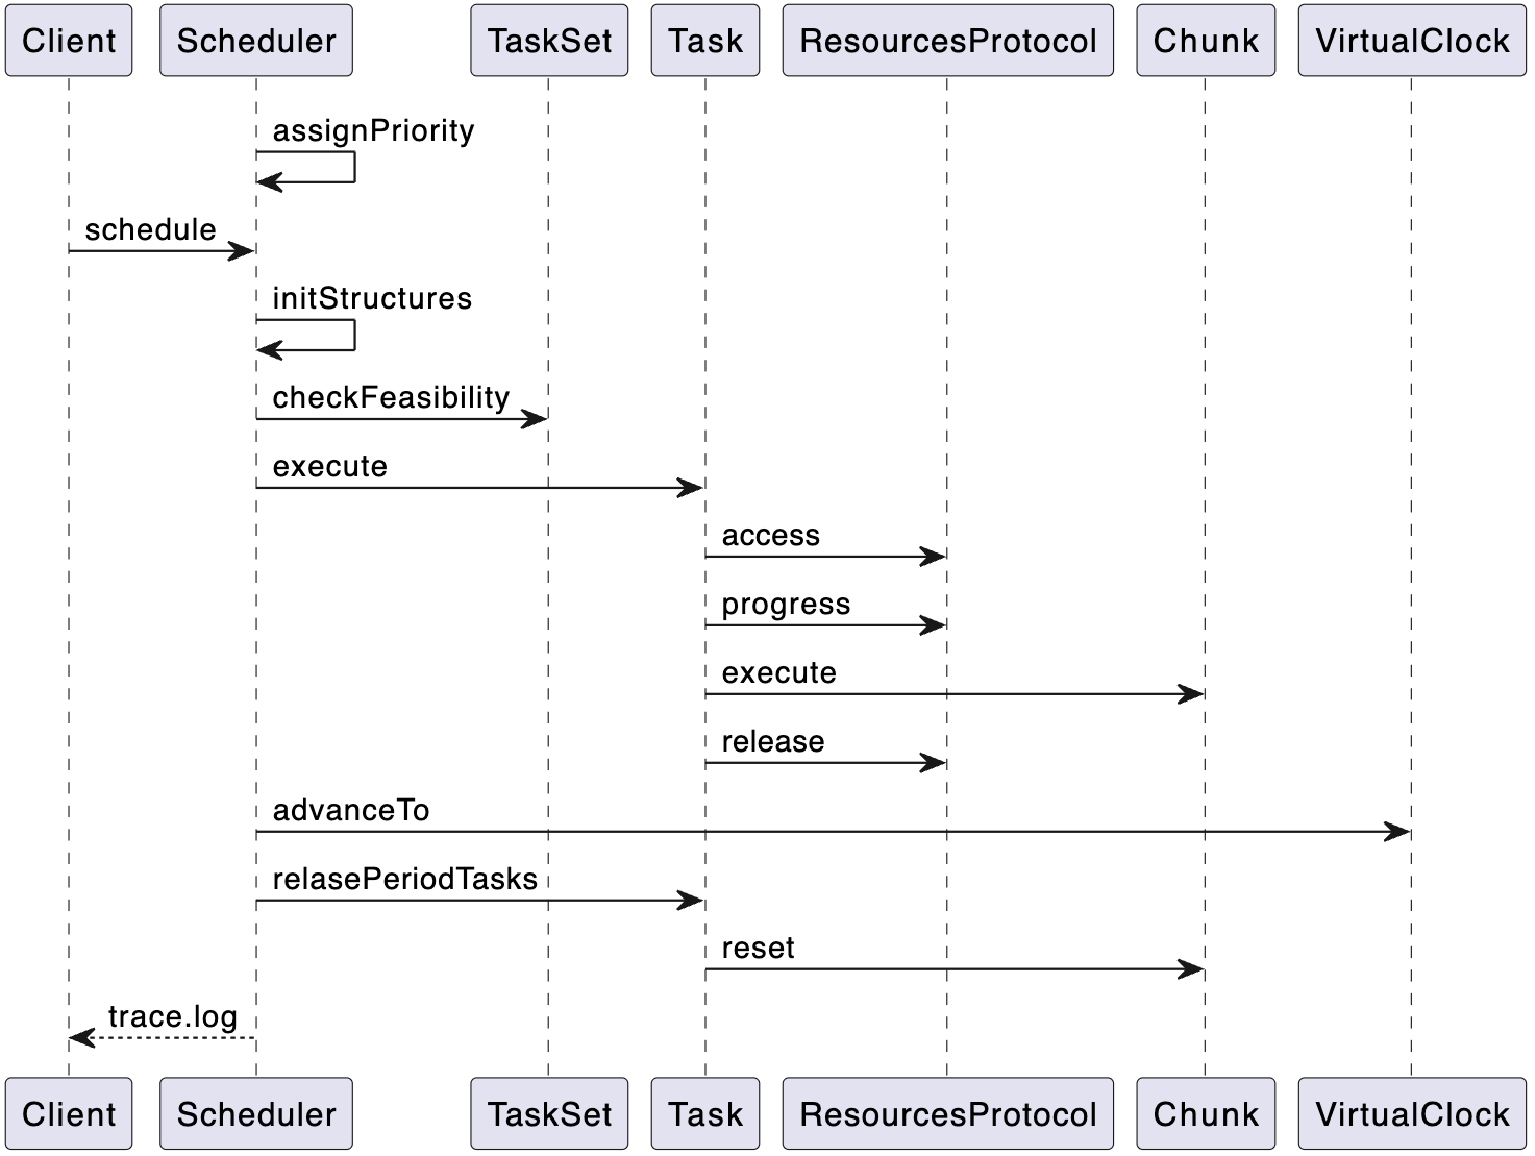
\includegraphics[width=.9\textwidth]{immagini/sequence diagram.pdf}
    \caption{Sequence Diagram scheduler}
    \label{fig:sequenceDiagram}
\end{figure}

\subsection{Rate Monotonic}
Vediamo come sono implementati i metodi astratti della classe \texttt{Scheduler} in RM, cioè quelli che definsicono il suo comportamento rispetto agli altri scheduler.
\begin{itemize}
    \item \texttt{checkFeasibility} \\
        Viene controllato l'hyperbolic bound. È stato deciso di non cnsiderare il test di Lui \& Layland viesto che questo non è tight: se un taskset non risulta schedulabile seconda questo test, l'hyperbolic bound potrebbe definire che è schedulabile.
    \item \texttt{assignPriority} \\
        Assegna la priorità in modo inverso rispetto alla durata del periodo.
    \item \texttt{addReadyTask} \\
        Siccome la lsita dei task pronti per l'esecuzione è oridnata in modo dinamica (visto che è implementata come un $TreeSet<Task>$ con un comparatore) secondo la priorità dinamica, aggiunge semplicemente il task a tale lista.
\end{itemize}

\subsection{Earlist Deadline First}
Vediamo come sono implementati i metodi astratti della classe \texttt{Scheduler} in EDF, cioè quelli che definsicono il suo comportamento rispetto agli altri scheduler.
\begin{itemize}
    \item \texttt{checkFeasibility} \\
        Viene controllato che il fattore di utilizzo del taskset sia minore o uguale a 1.
    \item \texttt{assignPriority} \\
        Assegna la priorità in modo inverso rispetto alla durata della dealine.
    \item \texttt{addReadyTask} \\
        Aggiunge il task alla lista dei task printi e poi la riordina secondo la prossima deadline. Il metodo che stabilisce la prossima deadline è \texttt{Task.nextDeadline}.
\end{itemize}

\subsection{Test}
Consideriamo situazioni diverse:
\begin{itemize}
    \item Schedulabile, senza risorse \\
        Il test esegue l'hyperbolic bound test che passa; siccome il test è sufficiente sappiamo che la sua accettazione ci assicura che il taskset sia schedulabile da RM. A questo punto oltre a verificare che schedulare il taskset non sollevi un'eccezione, è stata valutata a mano la sequenza di tracce generata.
    \item Non schedulabile, senza risorse \\
        È stato preso in questo caso un taskset con fattore di utilizzo maggiore di 1: in questo modo sicuramente la schedulabilità non deve passare. Dopo aver verficato che l'hyperbolic test non passi, verifichaimo che vengano sollevate le corrette eccezioni.
    \item Schedulabile e non schedulabile, con risorse \\
        Sono state presi dei task generati tramite chatGPT. Ci siamo accertati che quello generato dal modello di OpenAI rispetti quanto detto vericando il sollevamento o meno di eccezioni. Potrebbero essere implementati i test di schedulabilità estesi per risovere questo problema.
\end{itemize}


%%%%%%%%%%%%%%%%%%%%%%%%%%%%%%%%%%%%%%%%%%%%%%%%%%%%%%%%%%%%
\section{Resource Access Protocol}
\label{sec:resaccprot}
Ogni implementazione di un protocollo di accesso alle risorse deve estendere la classe \texttt{ResourceProtocol}.

l'idea iniziale era di implementare il concetto astratto di protocollo di accesso tramite un'interfaccia, ma vista la necessità di mantenere un riferimento allora scheduler nel protocollo si è introddo questo campo nella classe base.

\myskip

I metodi definiti da questa classe astratta sono le operazioni che devono essere svolte da un procotollo di questo tipo: deve gestire la fase di accesso, progresso e rilascio. Definisce anche il metodo \texttt{initStructures} che ha il compito di inizializzare le strutture dati usate dal protocollo.

Oltre a questi metodi è dichiarato un metodo \texttt{initStructures} che inizializza le strutture necessarie al protocollo.

\subsection{Priority Ceiling Protocol}
Tralasciando quello che fanno i metodi di accesso, progresso e rilascio, che riflettono quanto ci dice la teoria, in questo classe le strutture usate sono prevalentemente due:
\begin{itemize}
    \item \texttt{ceiling} \\
        È una mappa che associata ad ogni risorsa il suo ceiling, cioè la massima priorità nominale dei task che usano quella risorsa.
    \item \texttt{busyResources}\\
        È una lista delle risorse che sono occupate da un qualche task.
\end{itemize}

%%%%%%%%%%%%%%%%%%%%%%%%%%%%%%%%%%%%%%%%%%%%%%%%%%%%%%%%%%%%
\section{Fault injection}
Per implementare il fault injection di un additional execution time in un \texttt{chunk} è stato previsto un altro costruttore che prendesse, oltre ai parametri previsti, anche un \texttt{overheadExectutionTime}.

Il motivo per non introdurre una classe che eseguisse l'injection è stato che un chunk nella realtà nasce con il suo execution time e non ci sono altre entità che aumentano quello campionato; il costrutture vuole modellare questa idea.

%%%%%%%%%%%%%%%%%%%%%%%%%%%%%%%%%%%%%%%%%%%%%%%%%%%%%%%%%%%%
\section{Utilità}
Vediamo la scelta su alcuni componenti di utilità.

\subsection{Loggin}
Per il logging è stato implementato un semplice logging su un file e viene rappresnetato come una sequenza di coppie $<evento,tempo>$.

Il file di destinazione delle tracce loggate è \texttt{trace.log}.

\subsection{Clock}
Il tempo all'interno del sistema è gestito globalmente: ad ogni esecuzione del \texttt{main} il tempo viene resettato. Questa scelta è dovuta al fatto che praticamente tutti gli ogegtti devono accedere al clock del sistema; in questo modo si evita di passarlo ogni volta nei vari metodi chiamati a cascata. L'implementazione è stata fatta tramite il pattern Singleton.

A causa della staticità si consiglia di usare eseguire una sola simulazione per esecuzione. C'è la possibilità di resettarlo manualmente (tramite \texttt{MyClock.reset()}); questa possibilità è stata introdotto per i test.

Il clock del sistema è rappresnetato dalla classe \texttt{MyClock}. Questa non fa altro che mantenere il tempo assoluto ed esporre due metodi che permettono di avanzare di un dato intervallo temporale e avanzare fino a un determinato tempo.

\myskip

Il tempo è gestito tramite oggetti di tipo \texttt{Duration}, classe di \texttt{java.time} che implementa oggetti immutabili e che permetto una facile gestione del tempo.

In particolare il tempo deve essere consdierato dall'utente (i.e., passato in input e restituito poi in output) in millesecondi, ma il sistema lo gestisce tramite i nanosecondi. Questo permette di lavorare con millisecondi frazionari quando si campiona dalle distribuzioni di Sirio.

La stampa all'interno delf ile di log \texttt{trace.log} nel formato corretto è implementa nel metodo \texttt{Utils.printCurrentTime}.

\subsection{Sampling dei tempi}
Quando si deve definire i tempi che definiscono i vari componenti del sistema, cioè come il periodo, la dealine, l'execution time di un chunk, si usa un campionamento da un data distribuzione.

Le distribuzioni sono implementate dalla libreria \texttt{Sirio}; oltre a quelle definite dalla libreria è stata implementata la classe \texttt{ConstantSampler}, che permette di gestire tempi costanti, mantenendo l'astrazione della libreria Sirio.

\myskip

I sampler di Sirio restiuiscono oggetti di tipo \texttt{BigDecimal}. Come detto nel paragrafo sopra il sistema gestisce il tempo come oggetti di tipo \texttt{Duration}. Per implementare questo meccanismo è stata implementata la classe \texttt{SampleDuration}, che preso un \texttt{Sampler} restituisce il rispettivo tempo in nanosecondi.

\subsection{Eccezioni}
Durante l'esecuzione si possono verificare dei problemi, più o meno previsti. Questi sono gestiti tramite eccezioni; questo permette in futuro di cambiare o aggiungere un comportamente del sistema quando si verificano determinate situazioni.

\myskip

Le eccezioni implementate è utili sono:
\begin{itemize}
    \item \texttt{DeadlineMissedExeption} \\
        Viene sollevata quando un task non rispetta la deadline. Il sistema non la gestisce, ma la propaga fino al main: in questo modo se e quando si verifica questo problema, viene stamapta in \texttt{trace.log} e la simulazione si arresta.
    \item \texttt{AccessResourceProtocolExeption} \\
        Viene sollevata quando un task viene bloccato dal metodo \texttt{access} del protocollo di accesso.
\end{itemize}